\section{Cell Tracking}

\begin{frame}{Definition}
    \begin{itemize}
          \item Extract cell lineages from embryo data.
          \item Reconstruct fates of all cells in the embryo.
    \end{itemize}
\end{frame}

\begin{frame}{Existing Work}
    Two approaches:
    \begin{enumerate}
          \item State space models.
          \item Tracking-by-Assignment
        \begin{itemize}
              \item Chain Graph Tracking
        \end{itemize}
    \end{enumerate}
\end{frame}

\begin{frame}{Hypotheses Graph}
    \begin{figure}
        \centering
        \begin{subfigure}[b]{0.44\textwidth}
            \scalebox{0.62}{
                \begin{tikzpicture}[minimum size=58pt,scale=0.45, every node/.style={scale=0.45, text=black, font=\LARGE}, thick]
                        \begin{scope}
        \node (t1) {\huge $t$};
        \node[hypothesesdetection, below=of t1, circle, draw] (x11) {$X_1^t$};
        \node[hypothesesdetection, below=of x11, circle, draw] (x12) {$X_2^t$};
        \node[hypothesesdetection, below=of x12, circle, draw] (x13) {$X_3^t$};
    \end{scope}

    
    
    \begin{scope}
        \node[right=of t1, xshift=15mm] (t2) {\huge $t+1$};
        \node[hypothesesdetection, below=of t2, circle, draw] (x21) {$X_4^{t+1}$};
        \node[hypothesesdetection, below=of x21, circle, draw] (x22) {$X_5^{t+1}$};
    \end{scope}

    \begin{scope}[on background layer]
        \node[hypothesesdetection, below=of x22, circle, draw, on background layer] (x23) {$X_6^{t+1}$};
    \end{scope}
    
    
    \begin{scope}
        \node[right=of t2, xshift=15mm] (t3) {\huge $t+2$};
        \node[hypothesesdetection, below=of t3, circle, draw] (x31) {$X_7^{t+2}$};
        \node[hypothesesdetection, circle, draw, shift=($(x31.center)-(x21.center)$)] (x32) at (x22) {$X_8^{t+2}$};
    \end{scope}
    
    \begin{scope}[on background layer]
        \node[hypothesesdetection, below=of x32, circle, draw, on background layer] (x33) {$X_{10}^{t+2}$};
    \end{scope}
    
    % \begin{scope}
    %     \node[right=of t3, xshift=15mm] (t4) {\huge $t+3$};
    %     \node[hypothesesdetection, below=of t4, circle, draw] (x41) {$X_{10}^{t+3}$};
    %     \node[hypothesesdetection, below=of x41, circle, draw] (x42) {$X_{11}^{t+3}$};
    %     \node[hypothesesdetection, below=of x42, circle, draw] (x43) {$X_{12}^{t+3}$};
    % \end{scope}

    \begin{scope}[on background layer]
        \node[rectangle, draw, color=hypothesesbackground!40, fill=hypothesesbackground!30,
        fit=(x11) (x12) (x13), inner sep=13mm] (b1) {};
        \node[rectangle, draw, color=hypothesesbackground!40, fill=hypothesesbackground!30,
        fit=(x21) (x22) (x23), inner sep=13mm] (b2) {};
        \node[rectangle, draw, color=hypothesesbackground!40, fill=hypothesesbackground!30,
        fit=(b2), shift=($(t3.center) - (t2.center)$), inner sep=-0.1mm] (b3) {};
        % \node[rectangle, draw, color=hypothesesbackground!40, fill=hypothesesbackground!30,
        % fit=(x41) (x42) (x43), inner sep=13mm] (b4) {};
    \end{scope}

    \path[hypothesestransition] (x11) edge (x21);
    \path[hypothesestransition] (x12) edge (x22);
    \path[hypothesestransition] (x13) edge (x22);
    % \path[hypothesestransition] (x13) edge (x23);

    \path[hypothesestransition] (x21) edge (x31);
    \path[hypothesestransition] (x21) edge (x32);
    \path[hypothesestransition] (x22) edge (x32);
    % \path[hypothesestransition] (x23) edge (x32);

    % \path[hypothesestransition] (x31) edge (x41);
    % \path[hypothesestransition] (x32) edge (x42);
    % \path[hypothesestransition] (x32) edge (x43);

%%% Local Variables: 
%%% mode: latex
%%% TeX-master: "../../../main"
%%% End: 



%%% Local Variables: 
%%% mode: latex
%%% TeX-master: "../../main"
%%% End: 

                \end{tikzpicture}
            }
        \end{subfigure}
        \hfill
        \begin{subfigure}[b]{0.44\textwidth}
            \scalebox{0.62}{
                \begin{tikzpicture}[minimum size=58pt,scale=0.45, every node/.style={scale=0.45, text=black, font=\LARGE}, thick]
                        \begin{scope}
        \node (t1) {\huge $t$};
        \node[hypothesesdetection, below=of t1, circle, draw] (x11) {$X_1^t$};
    \end{scope}
    \begin{scope}[on background layer]
        \node[hypothesesdetection, below=of x11, circle, draw] (x12) {$X_2^t$};
    \end{scope}
    \begin{scope}
        \node[hypothesesdetection, below=of x12, circle, draw] (x13) {$X_3^t$};
    \end{scope}

    
    
    \begin{scope}
        \node[right=of t1, xshift=15mm] (t2) {\huge $t+1$};
        \node[hypothesesdetection, below=of t2, circle, draw] (x21) {$X_4^{t+1}$};
        \node[hypothesesdetection, below=of x21, circle, draw] (x22) {$X_5^{t+1}$};
    \end{scope}

    \begin{scope}[on background layer]
        \node[hypothesesdetection, below=of x22, circle, draw, on background layer] (x23) {$X_6^{t+1}$};
    \end{scope}
    
    
    \begin{scope}
        \node[right=of t2, xshift=15mm] (t3) {\huge $t+2$};
        \node[hypothesesdetection, below=of t3, circle, draw] (x31) {$X_7^{t+2}$};
        \node[hypothesesdetection, circle, draw, shift=($(x31.center)-(x21.center)$)] (x32) at (x22) {$X_8^{t+2}$};
    \end{scope}
    
    \begin{scope}[on background layer]
        \node[hypothesesdetection, below=of x32, circle, draw, on background layer] (x33) {$X_{10}^{t+2}$};
    \end{scope}
    
    % \begin{scope}
    %     \node[right=of t3, xshift=15mm] (t4) {\huge $t+3$};
    %     \node[hypothesesdetection, below=of t4, circle, draw] (x41) {$X_{10}^{t+3}$};
    %     \node[hypothesesdetection, below=of x41, circle, draw] (x42) {$X_{11}^{t+3}$};
    %     \node[hypothesesdetection, below=of x42, circle, draw] (x43) {$X_{12}^{t+3}$};
    % \end{scope}

    \begin{scope}[on background layer]
        \node[rectangle, draw, color=hypothesesbackground!40, fill=hypothesesbackground!30,
        fit=(x11) (x12) (x13), inner sep=13mm] (b1) {};
        \node[rectangle, draw, color=hypothesesbackground!40, fill=hypothesesbackground!30,
        fit=(x21) (x22) (x23), inner sep=13mm] (b2) {};
        \node[rectangle, draw, color=hypothesesbackground!40, fill=hypothesesbackground!30,
        fit=(b2), shift=($(t3.center) - (t2.center)$), inner sep=-0.1mm] (b3) {};
        % \node[rectangle, draw, color=hypothesesbackground!40, fill=hypothesesbackground!30,
        % fit=(x41) (x42) (x43), inner sep=13mm] (b4) {};
    \end{scope}

    \path[hypothesestransition] (x11) edge (x21);
    % \path[hypothesestransition] (x12) edge (x22);
    \path[hypothesestransition] (x13) edge (x22);
    % \path[hypothesestransition] (x13) edge (x23);

    \path[hypothesestransition] (x21) edge (x31);
    % \path[hypothesestransition] (x21) edge (x32);
    \path[hypothesestransition] (x22) edge (x32);
    % \path[hypothesestransition] (x23) edge (x32);

    % \path[hypothesestransition] (x31) edge (x41);
    % \path[hypothesestransition] (x32) edge (x42);
    % \path[hypothesestransition] (x32) edge (x43);

%%% Local Variables: 
%%% mode: latex
%%% TeX-master: "../../../main"
%%% End: 



%%% Local Variables: 
%%% mode: latex
%%% TeX-master: "../../main"
%%% End: 

                \end{tikzpicture}
            }
        \end{subfigure}
        \caption{Hypotheses Graph for potential detections and assignments.}
        \label{fig:cell-tracking-hypotheses}
    \end{figure}
\end{frame}

\begin{frame}{Chain Graph Tracking}
    \begin{figure}
        \centering
        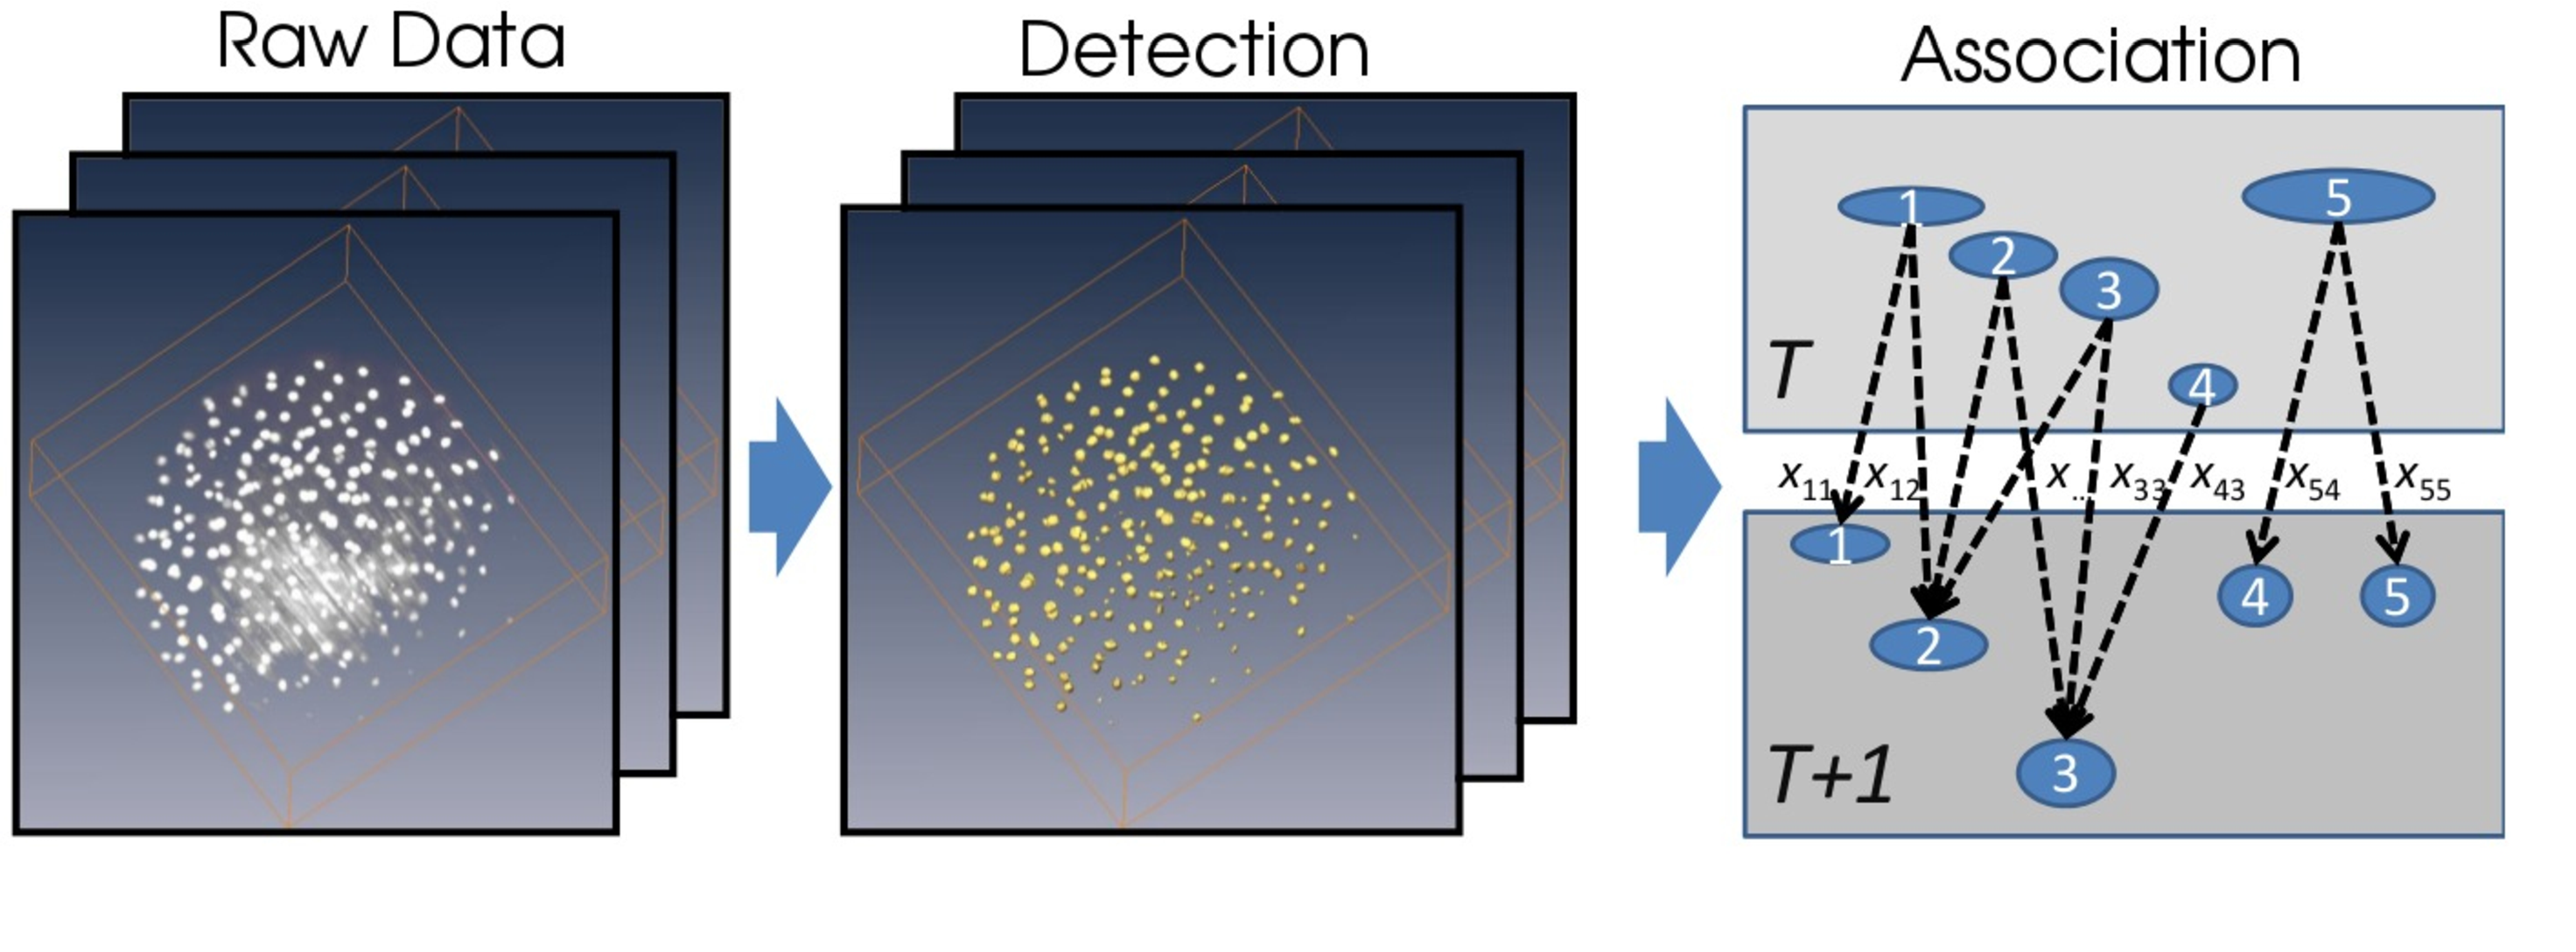
\includegraphics[width=\textwidth]{images/cell_tracking/pipeline.pdf}
        \caption{Chain graph tracking pipeline [SOURCE].}
        \label{fig:chaingraph-pipeline}
    \end{figure}
\end{frame}

\begin{frame}{Chain Graph Tracking}
    \begin{figure}
        \centering
        \begin{subfigure}[b]{0.44\textwidth}
            \centering
            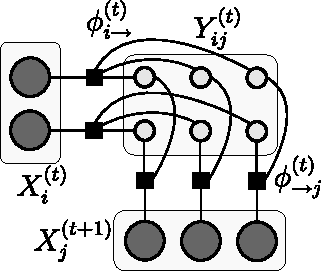
\includegraphics[width=\textwidth]{images/cell_tracking/fig_crf_less_nodes.pdf}
            \caption{CRF}
            \label{fig:chaingraph-crf}
        \end{subfigure}
        \hspace{5pt}
        \begin{subfigure}[b]{0.44\textwidth}
            \centering
            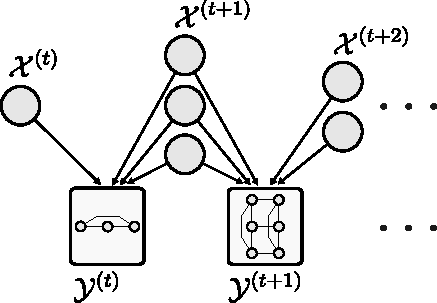
\includegraphics[width=\textwidth]{images/cell_tracking/fig_chain_graph.pdf}
            \caption{Chain Graph}
            \label{fig:chaingraph-cg}
        \end{subfigure}
        \caption{Chain graph model. [SOURCE]}
        \label{fig:chaingraph-model}
    \end{figure}
\end{frame}

\begin{frame}{Chain Graph Tracking}
    \begin{itemize}
          \item Can distinguish between cells and noise.
          \item Allows for tracking in oversegmented images.
          \item Fails in case of undersegmentation, that is in the presence of merged or overlapping objects.
    \end{itemize}
\end{frame}


%%% Local Variables: 
%%% mode: latex
%%% TeX-master: "../main"
%%% End: 
